\documentclass{article}

\usepackage{amsmath}
\usepackage{tabularx}
\usepackage[table]{xcolor}
\usepackage{hyperref}
\usepackage{cleveref}
\usepackage{tikz}
\usetikzlibrary{positioning, calc, shapes, arrows, fit}
\usepackage{circuitikz}
\usepackage{subcaption}
\usepackage[colorinlistoftodos]{todonotes}
\linespread{0.9}
\hypersetup{
    colorlinks = true,
    linkbordercolor = {black}
}
\begin{document}
\title{Lab 2 -- Using the Si5351 clock generator circuit with ItsyBitsy}
\author{
    Yifan Zhu\\
    Lab Partner: John Kustin
}
\maketitle

\begin{abstract}
    We use an ItsyBitsy to build a Si5352 clock generator circuit to generate waveforms at various frequencies.
\end{abstract}

\section{Introduction}
In various circuits we need ``clock signals'' at some precise frequency.
A modern solution is to use clock generator ICs, which have advantages of being low-cost, having reasonable performance, and being able to generate signals at different frequencies with a single IC.

In this lab we will generate clock signals using the
\href{https://cdn-shop.adafruit.com/datasheets/Si5351.pdf}{Si5351} IC,
and we will send the control $\text{I}^2\text{C}$ signals to the Si5351 using the \href{https://learn.adafruit.com/introducing-adafruit-itsybitsy-m4}{ItsyBitsy} microcontroller and CircuitPython.

\section{Experimental Setup}

We did the assembly following the instructions \href{https://learn.adafruit.com/adafruit-si5351-clock-generator-breakout/overview}{online at adafruit}, while replacing the pinout for the Arduino microcontroller with that of the ItsyBitsy microcontroller:

\begin{enumerate}
    \item We soldered pins onto the ItsyBitsy and the Si5351 breakout board.
    \item We soldered SMA connectors onto the Si5351 breakout board.
          SMA connectors are needed to carry the generated clock signals that are essentially RF.
    \item According to the documentation of \href{https://learn.adafruit.com/adafruit-si5351-clock-generator-breakout/pinouts}{Adafruit Si5351 Breakout Board} and \href{https://cdn-learn.adafruit.com/downloads/pdf/introducing-adafruit-itsybitsy-m4.pdf}{ItsyBitsy}, using jumper wires we connected
          \begin{enumerate}
              \item the 3V pin (ItsyBitsy) to the Vin pin (Si5351 breakout),
              \item the GND pin (ItsyBitsy) to the GND pin (Si5351 breakout),
              \item the SCL pin (ItsyBitsy) to the SCL pin (Si5351 breakout),
              \item and the SDA pin (ItsyBitsy) to the SDA pin (Si5351 breakout).
          \end{enumerate}
    \item We updated the bootloader of the ItsyBitsy following the \href{https://learn.adafruit.com/introducing-adafruit-itsybitsy-m4/update-the-uf2-bootloader}{instructions}.
          And we installed CircuitPython following the instructions \href{https://learn.adafruit.com/introducing-adafruit-itsybitsy-m4/circuitpython}{here}.
    \item And the CircuitPython code is taken directly from the \href{https://learn.adafruit.com/adafruit-si5351-clock-generator-breakout/circuitpython}{Adafruit website}.
\end{enumerate}

\begin{figure}[h]
    \centering
    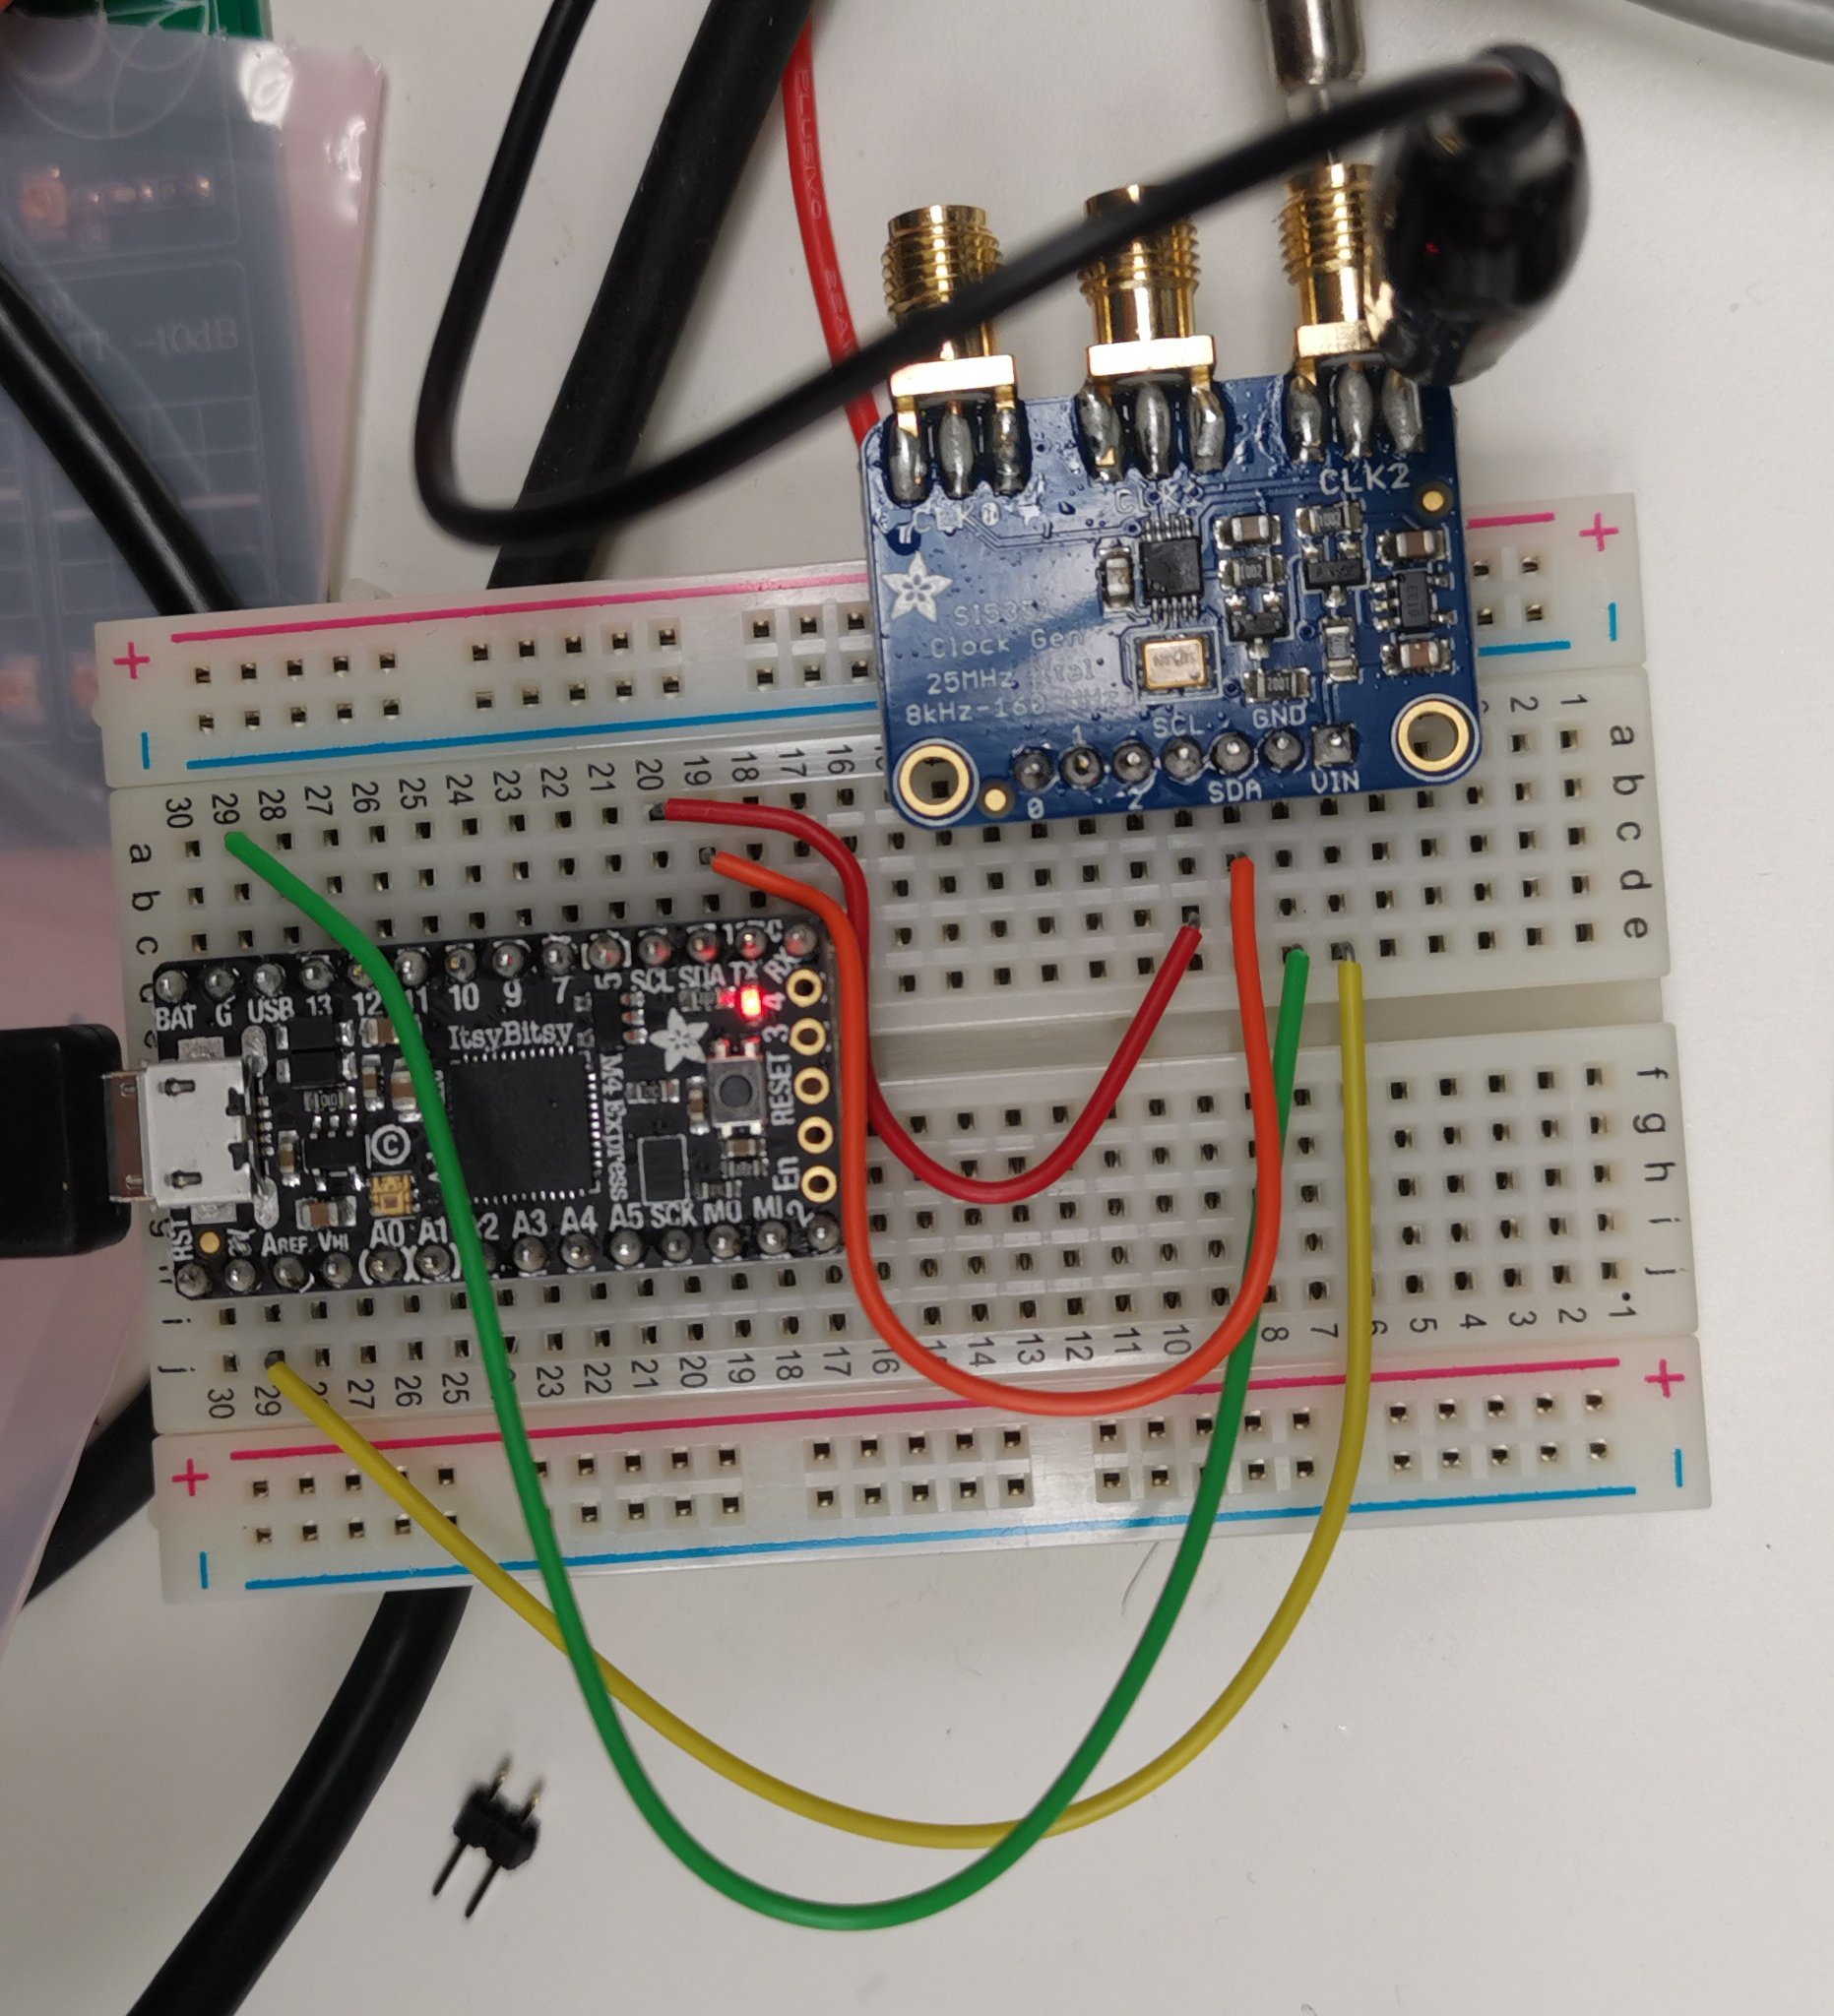
\includegraphics[width=.4\linewidth]{./pics/itsybitsy_si5351.jpg}
    \caption{Si5351 Clock Generator controlled By ItsyBitsy}
    \label{fig:assembly}
\end{figure}

The assembled circuit is shown in \Cref{fig:assembly}.

\section{Results}

The generated clock signals are shown in \Cref{fig:clock}.

\begin{figure}[h]
    \centering
    \begin{subfigure}{.33\linewidth}
        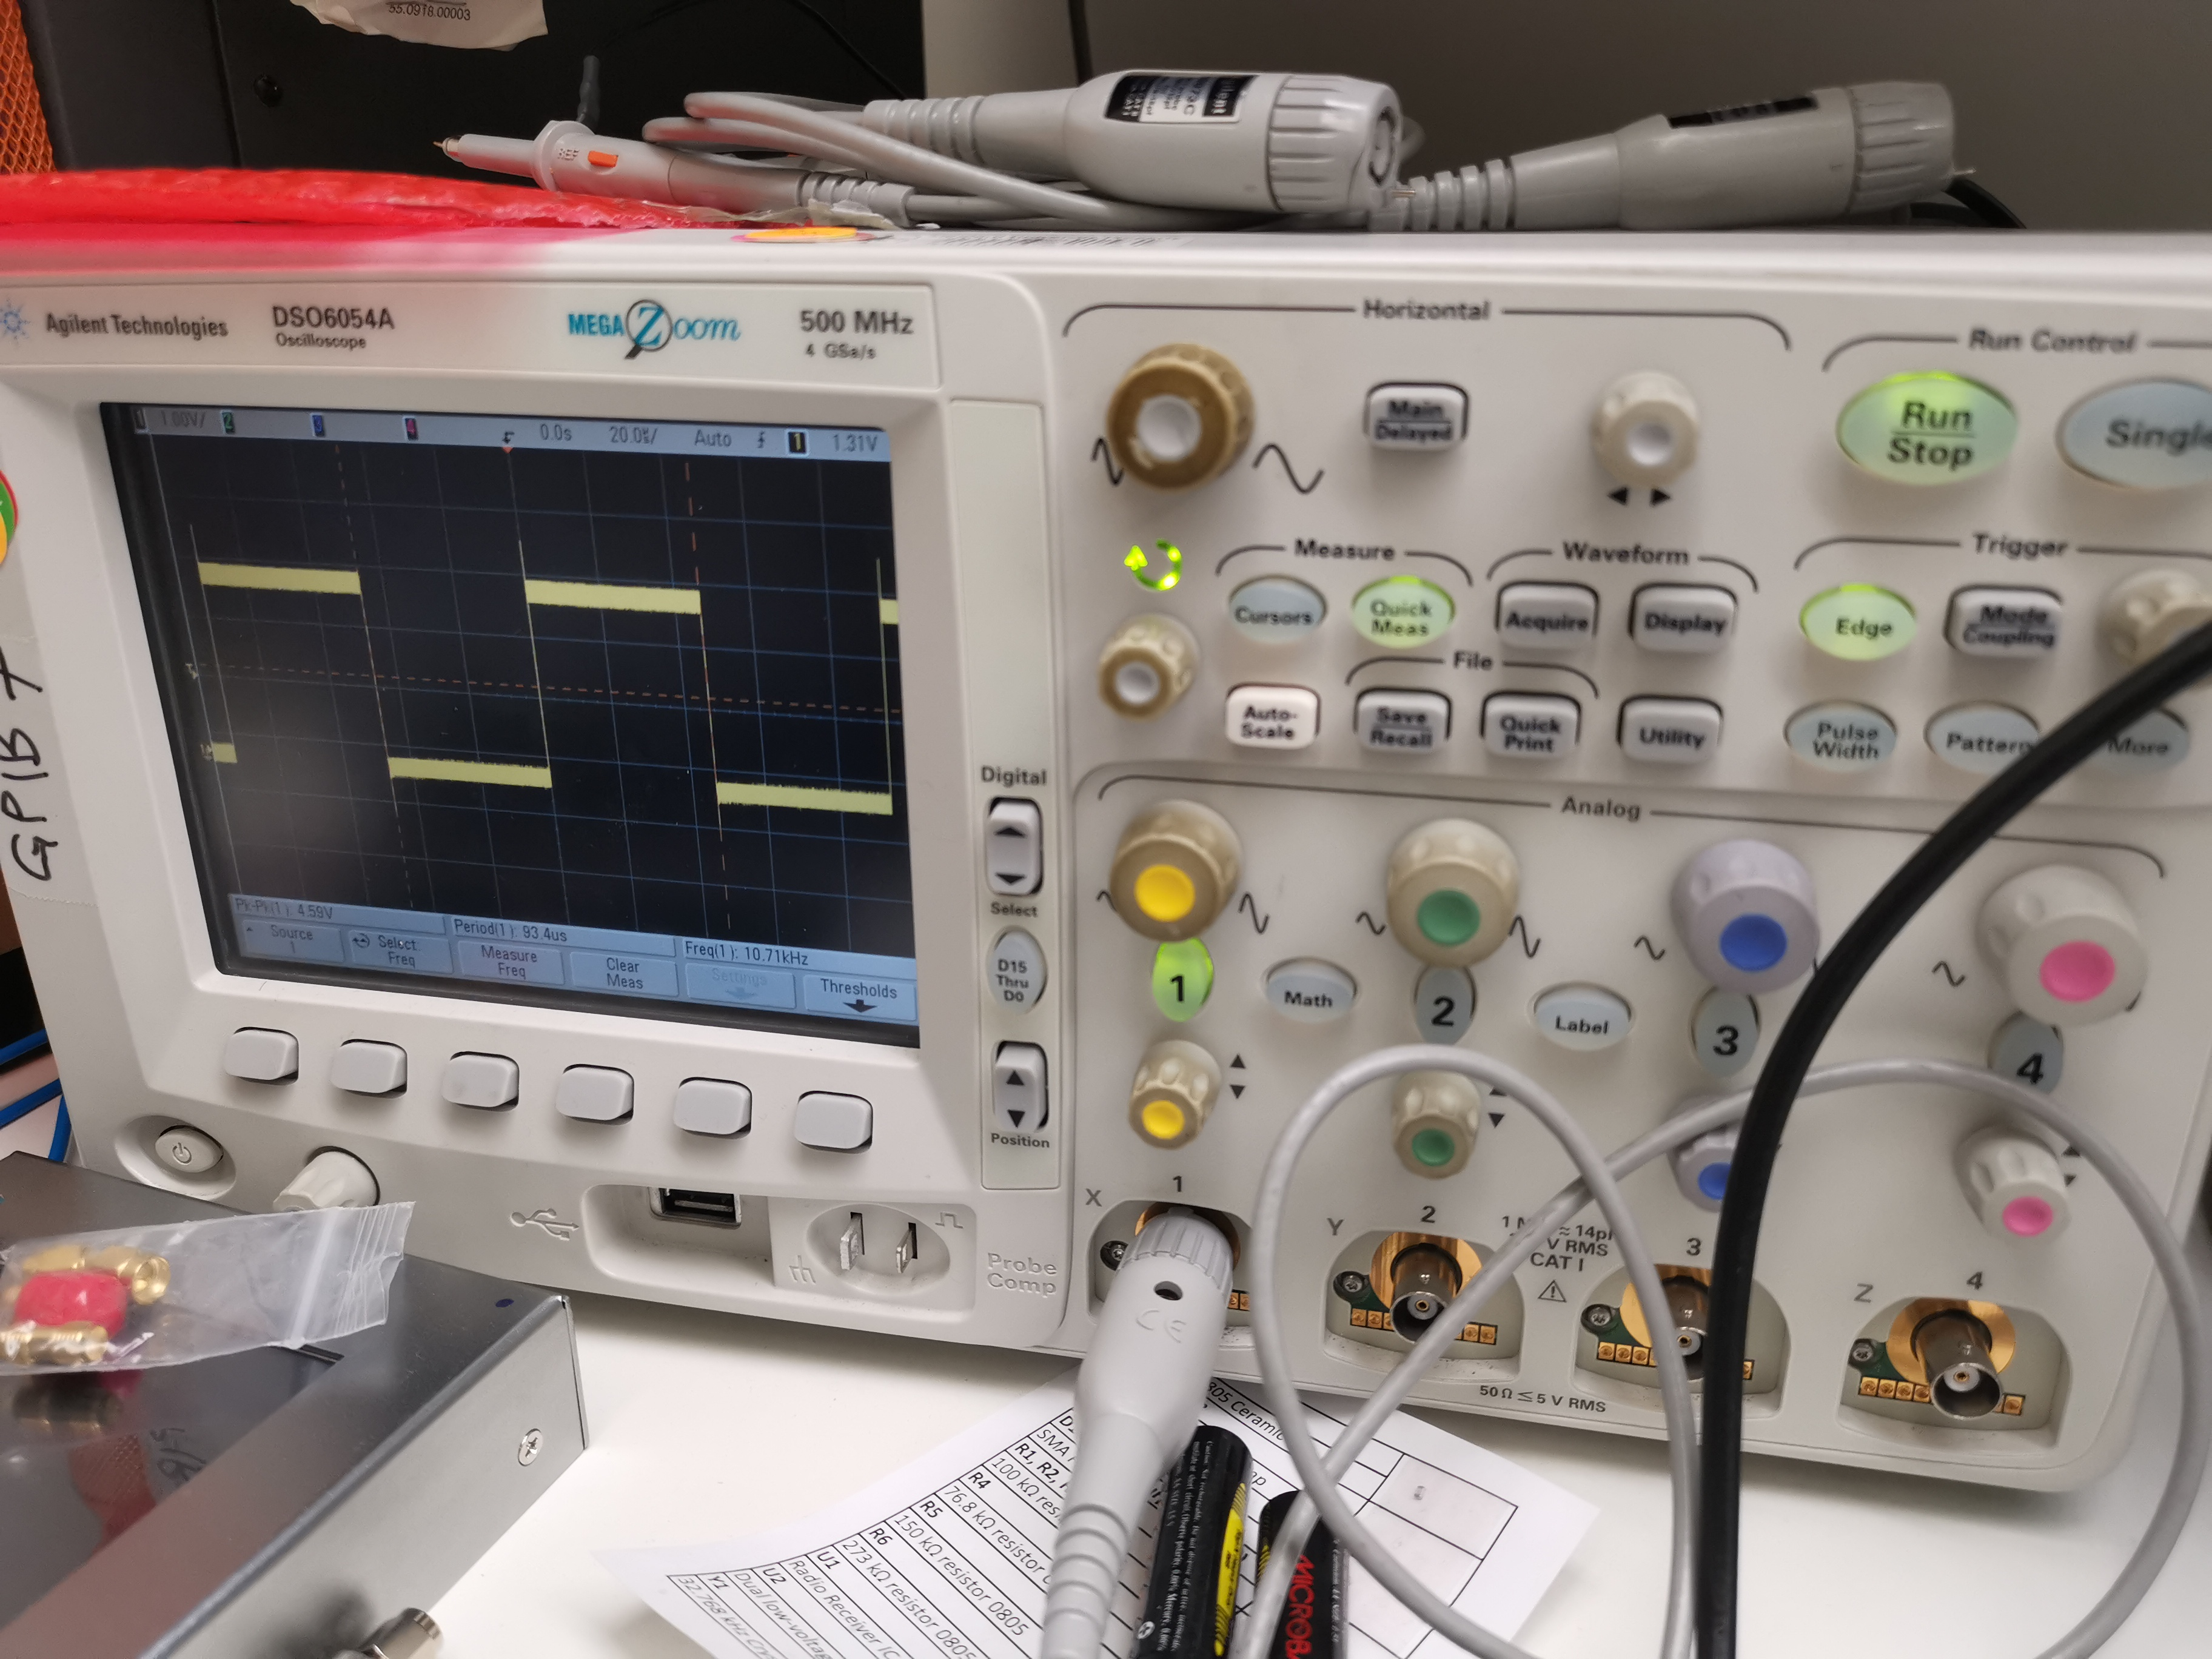
\includegraphics[width=.9\linewidth]{./pics/clock_10_70khz.jpg}
        \caption{10.706kHz generated clock signal}
        \label{fig:clock_10_70k}
    \end{subfigure}%
    \begin{subfigure}{.33\linewidth}
        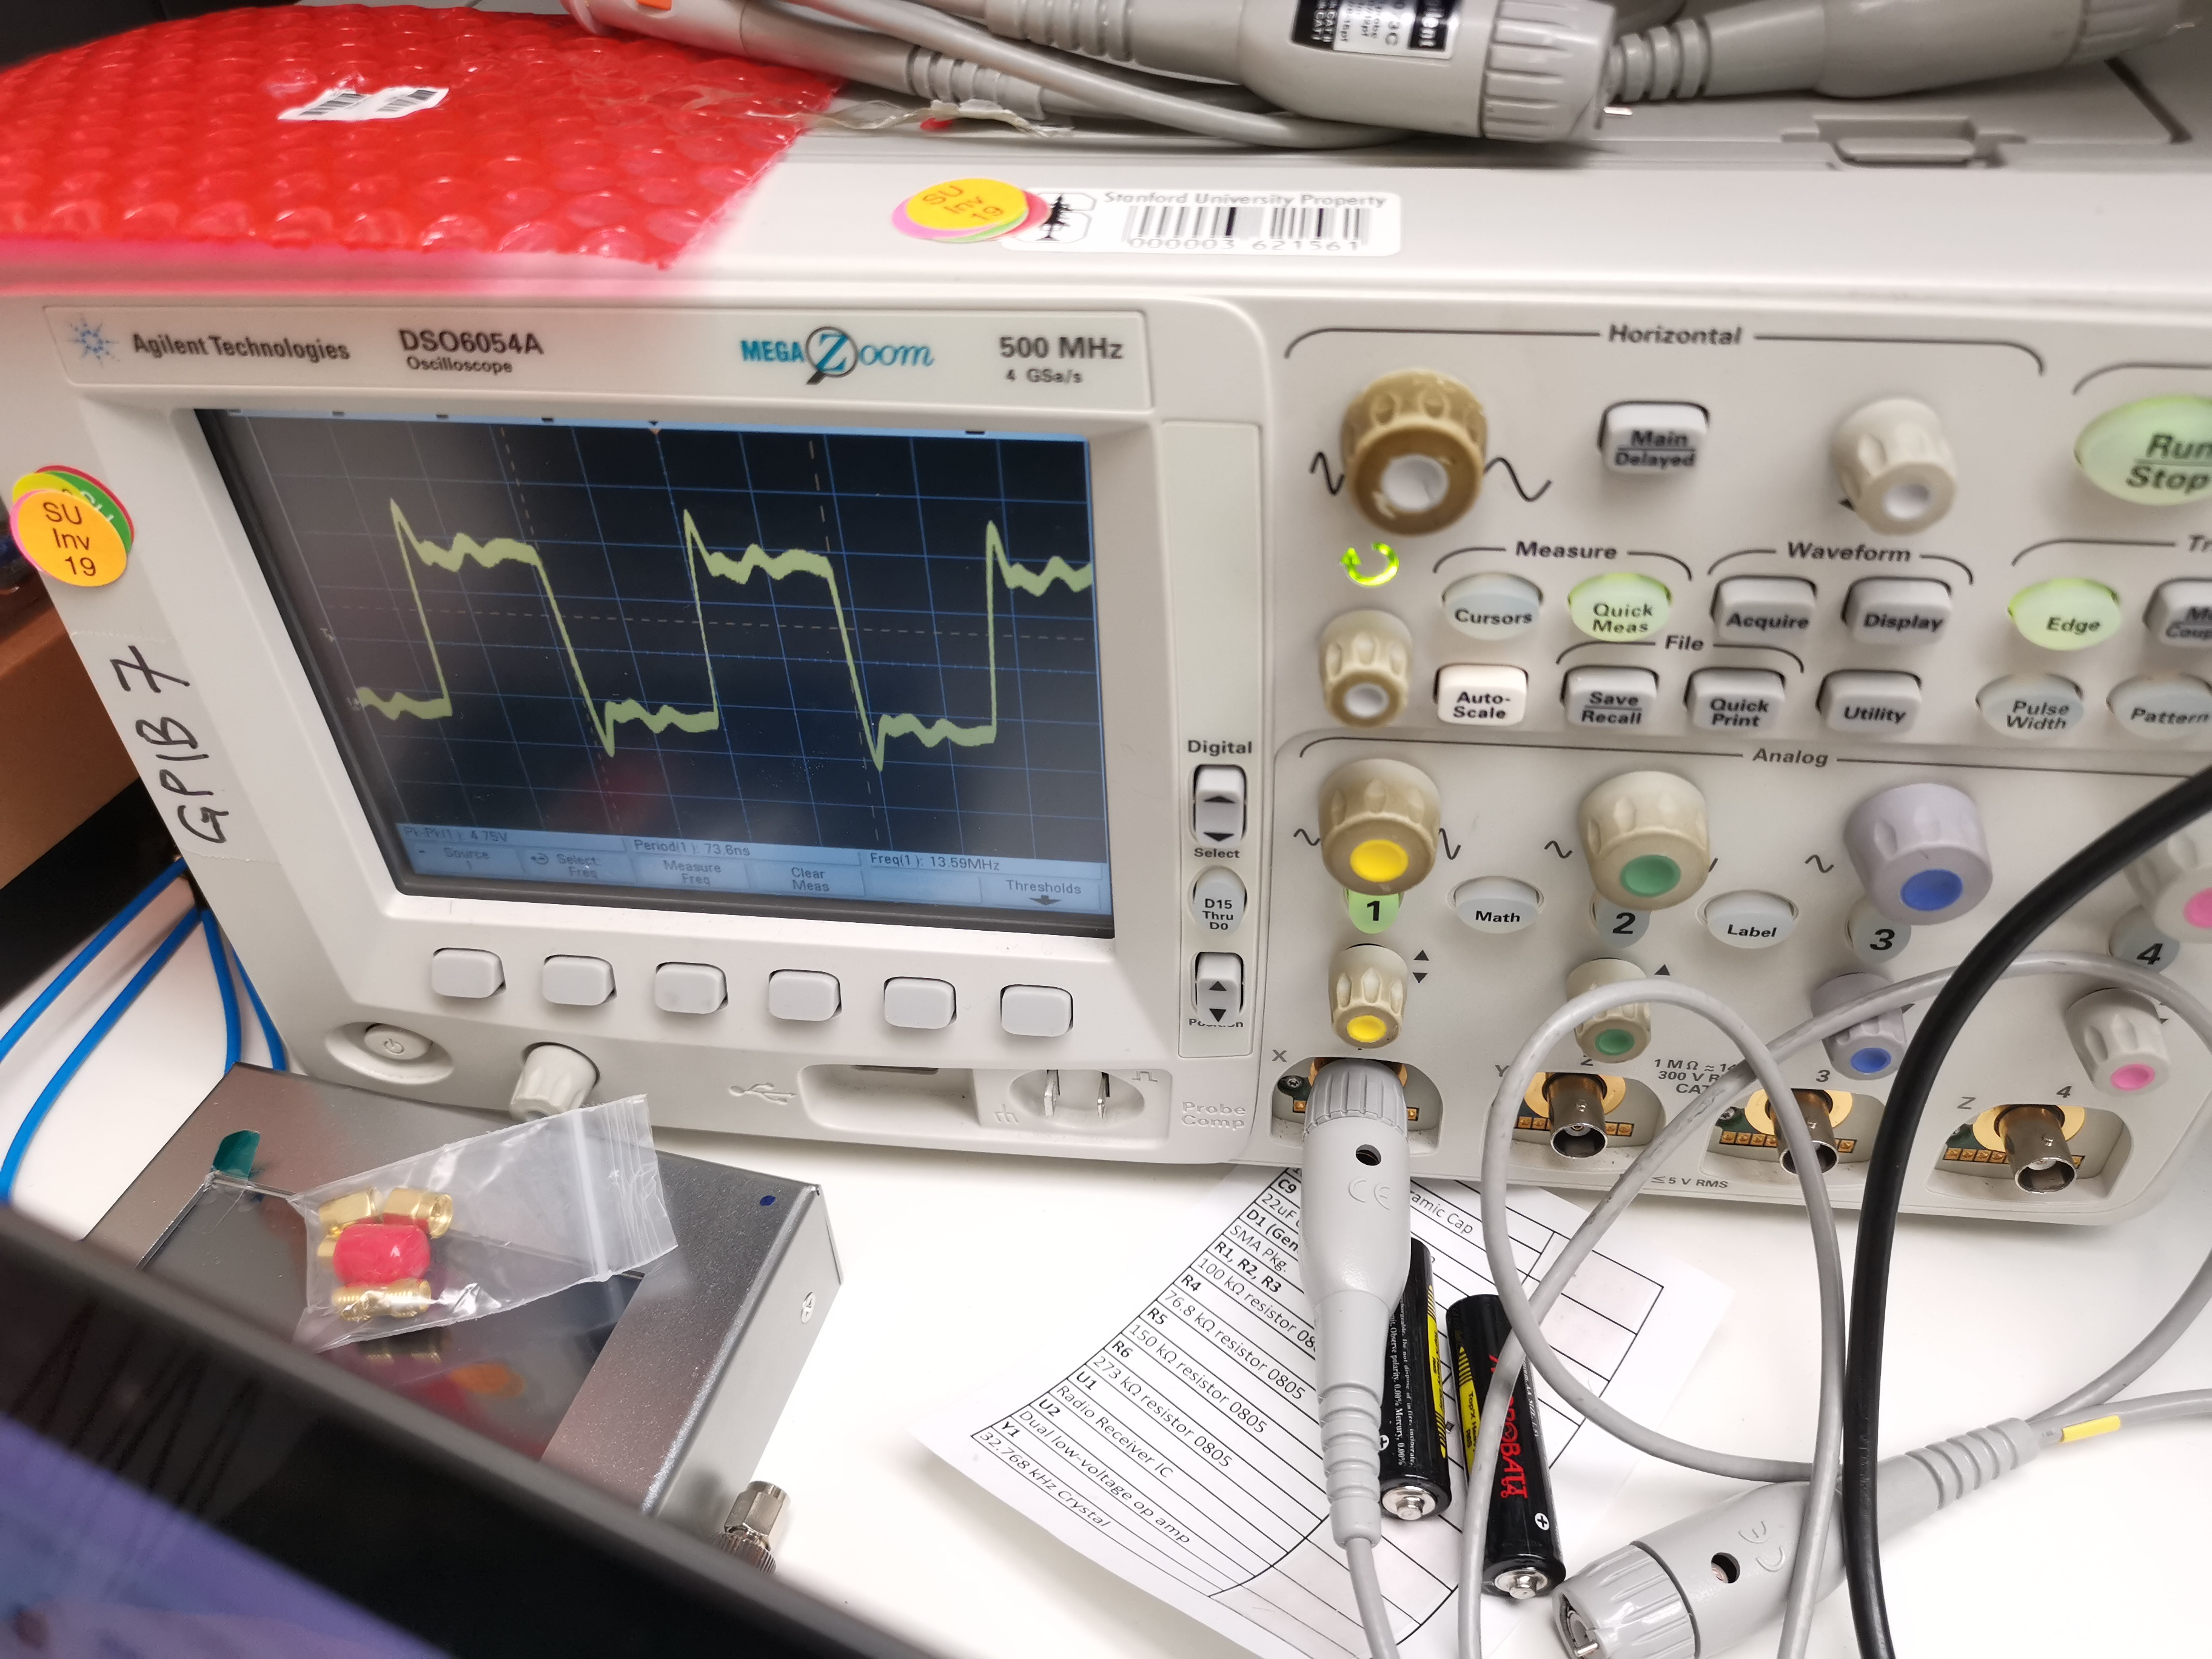
\includegraphics[width=.9\linewidth]{./pics/clock_13_55mhz.jpg}
        \caption{13.5531MHz generated clock signal}
        \label{fig:clock_13_55m}
    \end{subfigure}%
    \begin{subfigure}{.33\linewidth}
        \includegraphics[width=.9\linewidth]{./pics/clock_112_5mhz.jpeg}
        \caption{112.5MHz generated clock signal}
        \label{fig:clock_112_5m}
    \end{subfigure}%
    \caption{Generated Clock Signals at Various Frequencies}
    \label{fig:clock}
\end{figure}

\section{Discussion}

\section{Conclusions}

\end{document}